\documentclass{article}
\usepackage{lmodern}
\usepackage[T1]{fontenc}
\usepackage{shapepar}
\usepackage{microtype}
\usepackage{lipsum}
\usepackage{pgfplots}
\pgfplotsset{compat=1.9}
\usepackage{tikz}
\usetikzlibrary{calc,fit,intersections,folding}
\usepackage{pstricks-add}
\usetikzlibrary{arrows.meta,angles,arrows,quotes,backgrounds,calc}
\usepackage[left = 5mm, right = 5mm, top = 5mm, bottom = 5mm]{geometry}


\newcommand{\offsetx}{0.4}
\newcommand{\offsety}{0.6}

\newcommand{\cube}{
    \foreach\x in {0,1} {
        \foreach\y in {0,1} {
            \foreach\z in {0,1} {
                \coordinate (\x\y\z) at (\x+\offsetx*\z, \y+\offsety*\z);
            }
        }
    }
    \foreach\x in {0} {
        \foreach\y in {0,1} {
            \foreach\z in {0,1} {
                \draw[very thin] (\x\y\z) -- (1\y\z);
            }
        }
    }
    \foreach\x in {0,1} {
        \foreach\y in {0} {
            \foreach\z in {0,1} {
                \draw[very thin] (\x\y\z) -- (\x1\z);
            }
        }
    }
    \foreach\x in {0,1} {
        \foreach\y in {0,1} {
            \foreach\z in {0} {
                \draw[very thin] (\x\y\z) -- (\x\y1);
            }
        }
    }
}


\setlength{\parindent}{0em}

\newcommand{\clrone}{blue}
\newcommand{\clrtwo}{green!90!black}
\newcommand{\clrthree}{red!90!black}

\newcommand{\xshft}{2cm}
\newcommand{\yshft}{-3cm}

\begin{document}
\thispagestyle{empty}

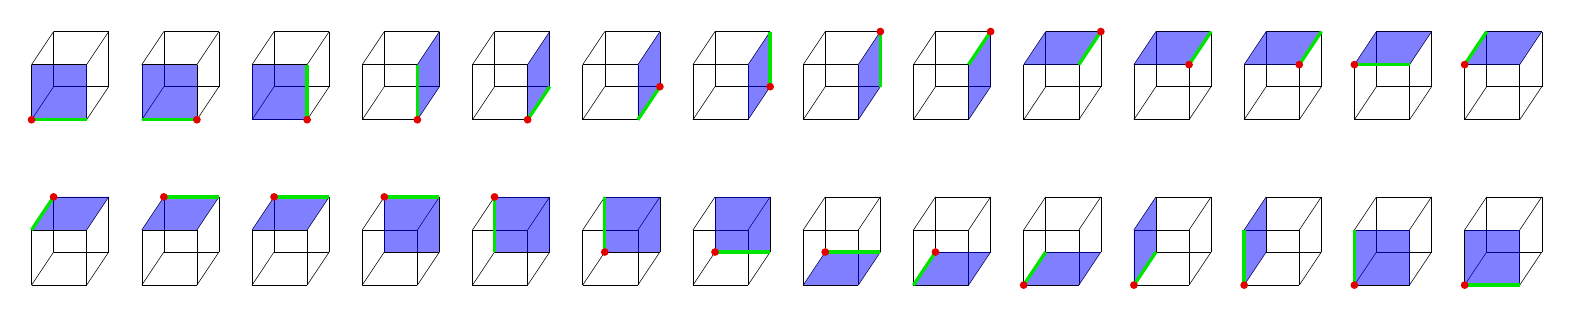
\begin{tikzpicture}[scale = 0.7]



\begin{scope}[xshift = 0*\xshft, yshift = 0*\yshft]
    \cube
    \fill[\clrone, opacity = 0.5] (000) -- (100) -- (110) -- (010) -- cycle;
    \draw[\clrtwo, very thick] (000) -- (100);
    \fill[\clrthree] (000) circle (2pt);
\end{scope}
\begin{scope}[xshift = 1*\xshft, yshift = 0*\yshft]
    \cube
    \fill[\clrone, opacity = 0.5] (000) -- (100) -- (110) -- (010) -- cycle;
    \draw[\clrtwo, very thick] (000) -- (100);
    \fill[\clrthree] (100) circle (2pt);
\end{scope}
\begin{scope}[xshift = 2*\xshft, yshift = 0*\yshft]
    \cube
    \fill[\clrone, opacity = 0.5] (000) -- (100) -- (110) -- (010) -- cycle;
    \draw[\clrtwo, very thick] (100) -- (110);
    \fill[\clrthree] (100) circle (2pt);
\end{scope}
\begin{scope}[xshift = 3*\xshft, yshift = 0*\yshft]
    \cube
    \fill[\clrone, opacity = 0.5] (100) -- (110) -- (111) -- (101) -- cycle;
    \draw[\clrtwo, very thick] (100) -- (110);
    \fill[\clrthree] (100) circle (2pt);
\end{scope}
\begin{scope}[xshift = 4*\xshft, yshift = 0*\yshft]
    \cube
    \fill[\clrone, opacity = 0.5] (100) -- (110) -- (111) -- (101) -- cycle;
    \draw[\clrtwo, very thick] (100) -- (101);
    \fill[\clrthree] (100) circle (2pt);
\end{scope}
\begin{scope}[xshift = 5*\xshft, yshift = 0*\yshft]
    \cube
    \fill[\clrone, opacity = 0.5] (100) -- (110) -- (111) -- (101) -- cycle;
    \draw[\clrtwo, very thick] (100) -- (101);
    \fill[\clrthree] (101) circle (2pt);
\end{scope}
\begin{scope}[xshift = 6*\xshft, yshift = 0*\yshft]
    \cube
    \fill[\clrone, opacity = 0.5] (100) -- (110) -- (111) -- (101) -- cycle;
    \draw[\clrtwo, very thick] (101) -- (111);
    \fill[\clrthree] (101) circle (2pt);
\end{scope}
\begin{scope}[xshift = 7*\xshft, yshift = 0*\yshft]
    \cube
    \fill[\clrone, opacity = 0.5] (100) -- (110) -- (111) -- (101) -- cycle;
    \draw[\clrtwo, very thick] (101) -- (111);
    \fill[\clrthree] (111) circle (2pt);
\end{scope}
\begin{scope}[xshift = 8*\xshft, yshift = 0*\yshft]
    \cube
    \fill[\clrone, opacity = 0.5] (100) -- (110) -- (111) -- (101) -- cycle;
    \draw[\clrtwo, very thick] (110) -- (111);
    \fill[\clrthree] (111) circle (2pt);
\end{scope}
\begin{scope}[xshift = 9*\xshft, yshift = 0*\yshft]
    \cube
    \fill[\clrone, opacity = 0.5] (010) -- (110) -- (111) -- (011) -- cycle;
    \draw[\clrtwo, very thick] (110) -- (111);
    \fill[\clrthree] (111) circle (2pt);
\end{scope}
\begin{scope}[xshift = 10*\xshft, yshift = 0*\yshft]
    \cube
    \fill[\clrone, opacity = 0.5] (010) -- (110) -- (111) -- (011) -- cycle;
    \draw[\clrtwo, very thick] (110) -- (111);
    \fill[\clrthree] (110) circle (2pt);
\end{scope}
\begin{scope}[xshift = 11*\xshft, yshift = 0*\yshft]
    \cube
    \fill[\clrone, opacity = 0.5] (010) -- (110) -- (111) -- (011) -- cycle;
    \draw[\clrtwo, very thick] (110) -- (111);
    \fill[\clrthree] (110) circle (2pt);
\end{scope}
\begin{scope}[xshift = 12*\xshft, yshift = 0*\yshft]
    \cube
    \fill[\clrone, opacity = 0.5] (010) -- (110) -- (111) -- (011) -- cycle;
    \draw[\clrtwo, very thick] (010) -- (110);
    \fill[\clrthree] (010) circle (2pt);
\end{scope}
\begin{scope}[xshift = 13*\xshft, yshift = 0*\yshft]
    \cube
    \fill[\clrone, opacity = 0.5] (010) -- (110) -- (111) -- (011) -- cycle;
    \draw[\clrtwo, very thick] (010) -- (011);
    \fill[\clrthree] (010) circle (2pt);
\end{scope}
\begin{scope}[xshift = 0*\xshft, yshift = 1*\yshft]
    \cube
    \fill[\clrone, opacity = 0.5] (010) -- (110) -- (111) -- (011) -- cycle;
    \draw[\clrtwo, very thick] (010) -- (011);
    \fill[\clrthree] (011) circle (2pt);
\end{scope}
\begin{scope}[xshift = 1*\xshft, yshift = 1*\yshft]
    \cube
    \fill[\clrone, opacity = 0.5] (010) -- (110) -- (111) -- (011) -- cycle;
    \draw[\clrtwo, very thick] (011) -- (111);
    \fill[\clrthree] (011) circle (2pt);
\end{scope}
\begin{scope}[xshift = 2*\xshft, yshift = 1*\yshft]
    \cube
    \fill[\clrone, opacity = 0.5] (010) -- (110) -- (111) -- (011) -- cycle;
    \draw[\clrtwo, very thick] (011) -- (111);
    \fill[\clrthree] (011) circle (2pt);
\end{scope}
\begin{scope}[xshift = 3*\xshft, yshift = 1*\yshft]
    \cube
    \fill[\clrone, opacity = 0.5] (001) -- (101) -- (111) -- (011) -- cycle;
    \draw[\clrtwo, very thick] (011) -- (111);
    \fill[\clrthree] (011) circle (2pt);
\end{scope}
\begin{scope}[xshift = 4*\xshft, yshift = 1*\yshft]
    \cube
    \fill[\clrone, opacity = 0.5] (001) -- (101) -- (111) -- (011) -- cycle;
    \draw[\clrtwo, very thick] (001) -- (011);
    \fill[\clrthree] (011) circle (2pt);
\end{scope}
\begin{scope}[xshift = 5*\xshft, yshift = 1*\yshft]
    \cube
    \fill[\clrone, opacity = 0.5] (001) -- (101) -- (111) -- (011) -- cycle;
    \draw[\clrtwo, very thick] (001) -- (011);
    \fill[\clrthree] (001) circle (2pt);
\end{scope}
\begin{scope}[xshift = 6*\xshft, yshift = 1*\yshft]
    \cube
    \fill[\clrone, opacity = 0.5] (001) -- (101) -- (111) -- (011) -- cycle;
    \draw[\clrtwo, very thick] (001) -- (101);
    \fill[\clrthree] (001) circle (2pt);
\end{scope}
\begin{scope}[xshift = 7*\xshft, yshift = 1*\yshft]
    \cube
    \fill[\clrone, opacity = 0.5] (000) -- (100) -- (101) -- (001) -- cycle;
    \draw[\clrtwo, very thick] (001) -- (101);
    \fill[\clrthree] (001) circle (2pt);
\end{scope}
\begin{scope}[xshift = 8*\xshft, yshift = 1*\yshft]
    \cube
    \fill[\clrone, opacity = 0.5] (000) -- (100) -- (101) -- (001) -- cycle;
    \draw[\clrtwo, very thick] (000) -- (001);
    \fill[\clrthree] (001) circle (2pt);
\end{scope}
\begin{scope}[xshift = 9*\xshft, yshift = 1*\yshft]
    \cube
    \fill[\clrone, opacity = 0.5] (000) -- (100) -- (101) -- (001) -- cycle;
    \draw[\clrtwo, very thick] (000) -- (001);
    \fill[\clrthree] (000) circle (2pt);
\end{scope}
\begin{scope}[xshift = 10*\xshft, yshift = 1*\yshft]
    \cube
    \fill[\clrone, opacity = 0.5] (000) -- (010) -- (011) -- (001) -- cycle;
    \draw[\clrtwo, very thick] (000) -- (001);
    \fill[\clrthree] (000) circle (2pt);
\end{scope}
\begin{scope}[xshift = 11*\xshft, yshift = 1*\yshft]
    \cube
    \fill[\clrone, opacity = 0.5] (000) -- (010) -- (011) -- (001) -- cycle;
    \draw[\clrtwo, very thick] (000) -- (010);
    \fill[\clrthree] (000) circle (2pt);
\end{scope}
\begin{scope}[xshift = 12*\xshft, yshift = 1*\yshft]
    \cube
    \fill[\clrone, opacity = 0.5] (000) -- (100) -- (110) -- (010) -- cycle;
    \draw[\clrtwo, very thick] (000) -- (010);
    \fill[\clrthree] (000) circle (2pt);
\end{scope}
\begin{scope}[xshift = 13*\xshft, yshift = 1*\yshft]
    \cube
    \fill[\clrone, opacity = 0.5] (000) -- (100) -- (110) -- (010) -- cycle;
    \draw[\clrtwo, very thick] (000) -- (100);
    \fill[\clrthree] (000) circle (2pt);
\end{scope}
    
    
\end{tikzpicture}


\end{document}